\documentclass[11pt]{article}
\usepackage[utf8]{inputenc}
\usepackage[T1]{fontenc}
\usepackage[margin=2.5cm]{geometry}
\usepackage{amsmath,amssymb,amsthm,mathtools}
\usepackage{enumitem}
\usepackage{graphicx}
\usepackage{booktabs}
\usepackage{xcolor}
\usepackage{hyperref}
\hypersetup{colorlinks=true,linkcolor=blue!60!black,citecolor=blue!55!black,urlcolor=blue!60!black}

\theoremstyle{plain}
\newtheorem{theorem}{Theorem}[section]
\newtheorem{proposition}[theorem]{Proposition}
\newtheorem{lemma}[theorem]{Lemma}
\newtheorem{corollary}[theorem]{Corollary}
\theoremstyle{definition}
\newtheorem{assumption}{Assumption}
\theoremstyle{remark}
\newtheorem{remark}[theorem]{Remark}

\newcommand{\R}{\mathbb{R}}
\newcommand{\N}{\mathbb{N}}
\newcommand{\T}{\mathbb{T}}
\newcommand{\E}{\mathbb{E}}
\newcommand{\KL}{\mathrm{KL}}
\newcommand{\Ham}{\mathrm{Ham}}
\newcommand{\Siv}{\Sigma_{\mathrm{inv}}}
\DeclareMathOperator*{\argmin}{arg\,min}
\DeclareMathOperator*{\argmax}{arg\,max}
\DeclareMathOperator{\supp}{supp}
\DeclareMathOperator{\dimm}{dim}
\DeclareMathOperator{\Var}{Var}

\title{\textbf{Adaptive exact minimax rates for invariant density\\
estimation on quotient spaces}}
\author{J.~Nemb\'e}
\date{\today}

\begin{document}
\maketitle

\begin{abstract}
We study nonparametric density estimation when the target is invariant under a
compact group $G$ acting on the sample space $E$. The orbit projection is
sufficient, so the problem reduces \emph{exactly} to density estimation on the
quotient $M=E/G$ of effective dimension $d=\dimm(E/G)=\dimm E-\dimm(\text{orbit})$.
We show that the minimax squared-Hellinger risk over the invariant H\"older class
$\Siv(s,L)$ is of order $n^{-2s/(2s+d)}$, with matching constants up to the rate:
a Fano lower bound built from $G$-invariant bumps on the quotient, paired with two
adaptive upper bounds. An orbital minimum-description-length (MDL) estimator
attains the rate up to a logarithmic factor; we prove this factor is a
\emph{coding artefact} and remove it with a penalised projection estimator that
attains the exact rate $n^{-2s/(2s+d)}$ adaptively in the unknown smoothness $s$.
The structural reason is isolated: a projection estimator pays the model's metric
complexity $D_k/n$, whereas a description-length code additionally pays the
per-coefficient quantisation cost $\log(1/\delta)\asymp\log n$. We then extend the
results to a \emph{multiplicative} (logarithmic-twin) regime---positive or
compositional data---where the Hellinger-affinity oracle step is tail-free, so the
gained rate persists on heavy-tailed data for which identity-coordinate
concentration is unavailable. We position the dimension-reduction phenomenon
against the recent ``exact sample-complexity gain from invariance'' literature and
delineate precisely what is a re-derivation and what is new.
\end{abstract}

\noindent\textbf{Keywords.} Invariant density estimation; minimax rates; group
action; quotient space; effective dimension; minimum description length;
penalised projection; adaptive estimation; Hellinger affinity.

\medskip
\noindent\textbf{MSC 2020.} 62G07, 62G20, 62C20.

\tableofcontents

\section{Introduction}\label{sec:intro}

\subsection{Problem and main result}

Let a compact group $G$ act on a sample space $E$, and suppose the unknown density
$f^\star$ of the i.i.d.\ data $X_1,\dots,X_n$ is \emph{$G$-invariant}:
$f^\star(g\cdot x)=f^\star(x)$ for all $g\in G$. Such structural priors are
ubiquitous: radial (rotation-invariant) densities, partially translation-invariant
fields, exchangeable or permutation-invariant models, and compositional data with
scale or sub-composition symmetries. The statistical question is how much the
invariance is worth.

A $G$-invariant density descends to a density $\tilde f^\star$ on the quotient
$M:=E/G$, a metric space of \emph{effective dimension}
\begin{equation}\label{eq:deff}
d:=\dimm(E/G)=\dimm E-\dimm(\text{generic orbit})=D-r ,
\end{equation}
where $D=\dimm E$ and $r$ is the dimension of a principal orbit. When $G$ acts
with \emph{positive-dimensional} orbits ($r>0$) the quotient is genuinely
lower-dimensional, and one expects the estimation rate to be governed by $d$ rather
than by $D$. Our main result makes this exact and adaptive.

\begin{theorem}[Exact adaptive minimax rate; informal]\label{thm:informal}
Under the standing assumptions of Section~\ref{sec:setting}, the minimax squared
Hellinger risk over the invariant H\"older ball $\Siv(s,L)$ satisfies
\[
\inf_{\widehat f}\ \sup_{f^\star\in\Siv(s,L)}\E\,h^2(P^\star,\widehat f)
\ \asymp\ n^{-2s/(2s+d)},\qquad d=\dimm(E/G).
\]
The lower bound holds for all $s>0$; the upper bound is attained, \emph{for the
exact rate and without knowledge of $s$}, by a penalised projection estimator on
the quotient. The invariant rate strictly improves on the non-invariant rate
$n^{-2s/(2s+D)}$ if and only if the orbits are positive-dimensional.
\end{theorem}

Two estimators appear. An \emph{orbital MDL} estimator---selecting a $G$-invariant
candidate density by minimising negative log-likelihood plus a Kraft code
length---attains the rate $(\log n/n)^{2s/(2s+d)}$, i.e.\ the minimax rate up to a
logarithmic factor. We then show that this $\log n$ is not intrinsic: it is the
per-coefficient cost of quantising a continuum into a prefix code. A penalised
projection estimator, which fits the coefficients without quantising them, pays
only the metric complexity of the model and attains the \emph{exact} rate,
adaptively.

\subsection{Contributions}

\begin{enumerate}[leftmargin=1.6em,label=(\arabic*)]
\item \textbf{A clean reduction and a complete lower bound.} We prove that the
orbit projection $\pi(X_i)$ is sufficient and that the invariant minimax risk
equals the minimax risk on the quotient (Lemma~\ref{lem:suff}), and we give a
self-contained Fano lower bound $n^{-2s/(2s+d)}$ using a Varshamov--Gilbert cube of
$G$-invariant bumps supported on the quotient (Theorem~\ref{thm:lower}).
\item \textbf{An information-theoretic (MDL/Hellinger) upper bound.} A tail-free
Kraft/partition-function bound (Lemma~\ref{lem:partition}) yields a Hellinger
oracle inequality with \emph{no} tail or moment assumption; combined with a twin
Jackson estimate on the (possibly stratified) quotient it gives the adaptive rate
$(\log n/n)^{2s/(2s+d)}$ (Theorem~\ref{thm:upper}).
\item \textbf{Removal of the logarithmic factor.} We prove that a single-resolution
projection estimator attains $n^{-2s/(2s+d)}$ exactly for known $s$
(Proposition~\ref{prop:knowns}) and that a penalised projection estimator attains
it \emph{adaptively} (Theorem~\ref{thm:adaptive}), and we isolate the mechanism:
metric complexity $D_k/n$ versus the coding cost $\log(1/\delta)$ of the
description-length penalty (Remark~\ref{rem:mechanism}).
\item \textbf{A multiplicative / twin extension.} On positive or compositional data
in a logarithmic chart, the affinity oracle step is tail-free and the loss is a
change-of-variables invariant, so the exact rate persists on heavy-tailed data
where identity-coordinate concentration fails (Section~\ref{sec:mult}).
\item \textbf{Honest positioning.} We delineate which parts re-derive the known
``invariance lowers the effective dimension'' phenomenon and which are new
(Section~\ref{sec:related}).
\end{enumerate}

\subsection{Related work and novelty}\label{sec:related}

That invariance reduces the effective dimension of a learning problem, and that
the gain is governed by the dimension of the quotient, is by now well understood,
particularly in the $L^2$/Sobolev and kernel settings. Tahmasebi and Jegelka
\cite{tahmasebi2023} quantify the \emph{exact} sample-complexity gain from
invariances for kernel ridge regression on manifolds; Elesedy and Zaidi
\cite{elesedy2021} and Bietti, Venturi and Bruna \cite{bietti2021} give related
generalisation and approximation analyses for invariant/equivariant models.
Classical nonparametric density estimation on manifolds and quotient spaces
(Hendriks \cite{hendriks1990}, Pelletier \cite{pelletier2005}) already produces
rates governed by the intrinsic dimension. Against this background, the bare
statement of Theorem~\ref{thm:informal} in the $L^2$/Sobolev setting is a
re-derivation and we present it as such.

What we add is threefold. First, an \emph{information-theoretic} route: the rate
emerges from the Barron--Cover \cite{barroncover} Kraft partition-function bound in
Hellinger risk, rather than from RKHS spectra, and the resulting estimator is
adaptive by construction. Second, an explicit and rigorous account of the
\emph{logarithmic gap} between description-length coding (near-minimax) and
projection/penalised estimation (exactly minimax), via the Birg\'e--Massart theory
\cite{birgemassart98,massart}; this clarifies a point that is often elided when MDL
or sieve-MDL procedures are called ``minimax optimal''. Third, the
\emph{multiplicative / twin} regime (Section~\ref{sec:mult}): the invariance is
taken with respect to a group acting in a logarithmic (non-additive) chart and
smoothness is measured there, so the gain extends to positive/compositional and
heavy-tailed data, a regime outside the cited additive analyses. The
tail-freeness of the affinity bound (Lemma~\ref{lem:partition}) is what makes this
extension automatic.

\subsection{Notation and organisation}

We write $h^2(P,Q)=\tfrac12\int(\sqrt{p}-\sqrt q)^2\,d\mu$ for the squared
Hellinger distance, $H=\sqrt{h^2}$ for the Hellinger metric,
$\rho(f,g)=\int\sqrt{fg}\,d\mu\in(0,1]$ for the affinity (so $h^2=1-\rho$), and
$\KL$ for Kullback--Leibler divergence. Throughout $M=E/G$, $d=\dimm M$,
$\pi:E\to M$ is the quotient map, $\mu_G=\pi_*\mu$ the quotient reference measure,
and $\Sigma(s,L)$ the H\"older ball of order $s$ and radius $L$ on $M$, with
$\Siv(s,L)=\{\tilde f\circ\pi:\tilde f\in\Sigma(s,L)\}$ its invariant pullback.
Section~\ref{sec:setting} sets up the reduction; Section~\ref{sec:lb} proves the
lower bound; Section~\ref{sec:mdl} the MDL near-minimax upper bound;
Section~\ref{sec:exact} the exact-rate projection estimators;
Section~\ref{sec:main} assembles the matching rate and the examples;
Section~\ref{sec:mult} the multiplicative extension; Section~\ref{sec:sim} gives a
numerical illustration; Section~\ref{sec:disc} discusses the stratified case and
open points.

\section{Setting and reduction to the quotient}\label{sec:setting}

\begin{assumption}[Geometry and group]\label{ass:geo}
$(E,\rho_E)$ is a compact metric space (typically a compact Riemannian manifold of
dimension $D$). A compact group $G$ acts continuously on $E$ by isometries with
closed orbits; principal orbits have dimension $r$. The quotient $M=E/G$ carries
the \emph{infimum (orbital) metric}
\[
d_G([x],[y]):=\inf_{g\in G}\rho_E(x,\,g\cdot y),
\]
and has covering dimension $d=\dimm M=D-r$ for a smooth proper action.
\end{assumption}

\begin{assumption}[Reference measure and invariant class]\label{ass:class}
Fix a $G$-invariant base measure $\mu$ on $E$ with pushforward $\mu_G=\pi_*\mu$.
The target is $G$-invariant, $f^\star=\tilde f^\star\circ\pi$, with
$\tilde f^\star\in\Sigma(s,L)$ and $0<c_0\le\tilde f^\star\le C_1<\infty$ on a
region $U\subseteq M$ on which $(M,d_G,\mu_G)$ is Ahlfors $d$-regular:
$c_M^{-1}r^d\le\mu_G(B(x,r))\le c_M r^d$ for $x\in U$, $0<r\le r_0$.
\end{assumption}

\begin{assumption}[Stratified quotient with full-mass top stratum]\label{ass:strata}
The quotient decomposes as $M=M_0\sqcup S$, where the \emph{principal stratum}
$M_0$ is an open $d$-dimensional manifold on which $(M_0,d_G,\mu_G)$ is Ahlfors
$d$-regular (Assumption~\ref{ass:class}, with $U\Subset M_0$), and the singular
locus $S$ (non-principal orbit types) satisfies $\dimm S<d$, hence $\mu_G(S)=0$.
For a free action $S=\varnothing$ and $M$ is a compact $d$-manifold.
\end{assumption}

Assumption~\ref{ass:strata} is what makes the orbifold case rigorous: by
Ahlfors $d$-regularity any set of dimension $<d$ is $\mu_G$-null, so all
$L^2(\mu_G)$- and $\KL$-integrals---approximation, projection variance, and the
information radius of the lower bound---are computed on the regular top stratum
$M_0$, a genuine $d$-dimensional space. The only case it excludes is a target
whose smoothness interacts essentially with the singular strata (where the local
dimension drops); we return to this in Section~\ref{sec:disc}. Throughout,
``on $M$'' may be read ``on $M_0$''.

The invariance prior in Assumption~\ref{ass:class} is what makes the gain real:
without it, orbit projection estimates only the invariant part $\pi_*P^\star$ and
there is nothing to gain. The following lemma is the formal reduction.

\begin{lemma}[Sufficiency of the orbit projection]\label{lem:suff}
Let $\mathcal F_{\mathrm{inv}}$ be a family of $G$-invariant densities on $E$ and
$X_1,\dots,X_n\stackrel{\text{iid}}{\sim}P_f$, $f\in\mathcal F_{\mathrm{inv}}$.
Then $(\pi(X_1),\dots,\pi(X_n))$ is sufficient for $f$, is i.i.d.\ from
$\tilde P_{\tilde f}=\pi_*P_f$ on $(M,\mu_G)$, and
$h^2_E(P_f,P_g)=h^2_M(\tilde P_{\tilde f},\tilde P_{\tilde g})$. Consequently
\[
\inf_{\widehat f}\ \sup_{f\in\mathcal F_{\mathrm{inv}}}\E\,h^2_E(P_f,\widehat f)
\;=\;
\inf_{\widehat{\tilde f}}\ \sup_{\tilde f}\E\,h^2_M(\tilde P_{\tilde f},\widehat{\tilde f}).
\]
\end{lemma}

\begin{proof}
Invariance $f=\tilde f\circ\pi$ gives $f(X_i)=\tilde f(\pi(X_i))$, so the
likelihood factors through $\pi(X_i)$: this is sufficiency, and the pushforward of
an i.i.d.\ sample is i.i.d. For the Hellinger identity, invariant densities make
the affinity integrate to the quotient,
$\int_E\sqrt{fg}\,d\mu=\int_M\sqrt{\tilde f\tilde g}\,d\mu_G$. For the equality of
minimax risks, note that under any $P_f$ with $f$ invariant, the conditional law of
$X_i$ given $\pi(X_i)=o$ is the normalised $G$-invariant measure on the orbit
$\pi^{-1}(o)$, which does not depend on $f$: the within-orbit position is
\emph{ancillary} with $f$-free law. Hence the experiment $(X_{1:n};\{P_f\})$ is Le
Cam-equivalent to $(\pi(X_{1:n});\{\tilde P_{\tilde f}\})$ augmented by independent
$f$-free randomisation, and the two minimax risks coincide; squared Hellinger,
being invariant, is the same loss on both sides.
\end{proof}

Lemma~\ref{lem:suff} reduces every statement below to density estimation of
$\tilde f^\star$ on the $d$-dimensional space $(M,\mu_G)$ from $n$ i.i.d.\ samples.
We henceforth work on $M$ and write $f^\star$ for $\tilde f^\star$ when no
confusion arises.

\section{Lower bound}\label{sec:lb}

We construct a Varshamov--Gilbert cube of $G$-invariant perturbations supported on
the quotient and apply Fano's method.

Fix a $\mathcal C^\infty$ function $\psi:\R^d\to\R$ with
$\supp\psi\subseteq(0,1)^d$, $\int\psi=0$, $\|\psi\|_\infty\le1$,
$\|\psi\|_{\mathcal C^s}\le1$, $\|\psi\|_{L^2}>0$. Identifying $U$ with a Euclidean
cube and $\mu_G$ with Lebesgue measure up to $c_M$, for a bandwidth $h=1/m$ split
$U$ into $N\asymp c_M h^{-d}$ sub-cubes $\{U_j\}$ of side $h$ and centres $x_j$, and
set
\begin{equation}\label{eq:bumps}
\psi_j(x):=L\,h^s\,\psi\!\Big(\tfrac{x-x_j}{h}\Big),\qquad
\tilde f_\omega:=f_0+\sum_{j=1}^N\omega_j\psi_j,\quad \omega\in\{0,1\}^N,
\end{equation}
where $f_0\in\Sigma(s,L/2)$ is a fixed reference with $c_0\le f_0\le C_1$ on $U$.

\begin{lemma}[Admissibility]\label{lem:admiss}
For $h\le h_0$ (so $Lh^s\le c_0/2$), each $\tilde f_\omega$ is a probability
density and $\tilde f_\omega\in\Sigma(s,c_1L)$ for a constant $c_1=c_1(\psi)$.
\end{lemma}

\begin{proof}
$\int\psi_j=Lh^s h^d\int\psi=0$, so $\int\tilde f_\omega=1$; and
$|\sum_j\omega_j\psi_j|\le Lh^s\le c_0/2$, so $\tilde f_\omega\ge c_0/2>0$. The
bumps have disjoint supports and $\|\psi_j\|_{\mathcal C^s}\le L$; for disjoint
supports the $\mathcal C^s$ seminorm of the sum is the maximum over $j$, whence
$\|\tilde f_\omega\|_{\mathcal C^s}\le\|f_0\|_{\mathcal C^s}+L\le c_1L$.
\end{proof}

\begin{lemma}[Varshamov--Gilbert {\cite[Lem.~2.9]{tsybakov}}]\label{lem:vg}
For $N\ge8$ there is $\Omega\subseteq\{0,1\}^N$ with $|\Omega|\ge2^{N/8}$ and
$\Ham(\omega,\omega')\ge N/8$ for distinct $\omega,\omega'\in\Omega$. Fix such an
$\Omega$ and a base point $\omega^{(0)}\in\Omega$.
\end{lemma}

\begin{lemma}[Separation and information radius]\label{lem:sepkl}
For distinct $\omega,\omega'\in\Omega$,
\[
h^2(\tilde f_\omega,\tilde f_{\omega'})\ \ge\ c_2\,L^2h^{2s},\qquad
c_2=\tfrac{c_M\|\psi\|_{L^2}^2}{64\,C_1},
\]
and, with $P_\omega^{\otimes n}$ the sample law,
$\KL(P_\omega^{\otimes n}\|P_{\omega^{(0)}}^{\otimes n})=n\,\KL(\tilde f_\omega\|\tilde f_{\omega^{(0)}})\le c_3\,nL^2h^{2s}$.
\end{lemma}

\begin{proof}
$(\sqrt a-\sqrt b)^2\ge(a-b)^2/(4C_1)$ since
$\tilde f_\omega,\tilde f_{\omega'}\in[c_0/2,2C_1]$. Disjoint supports give
$\int(\tilde f_\omega-\tilde f_{\omega'})^2=\Ham(\omega,\omega')L^2h^{2s+d}\|\psi\|_{L^2}^2$,
so $h^2\ge\tfrac1{8C_1}\Ham\cdot L^2h^{2s+d}\|\psi\|_{L^2}^2\ge c_2L^2h^{2s}$ using
$\Ham\ge N/8\asymp c_Mh^{-d}/8$. For the divergence,
$\KL\le\chi^2\le\tfrac2{c_0}\int(\tilde f_\omega-\tilde f_{\omega^{(0)}})^2\le\tfrac2{c_0}NL^2h^{2s+d}\|\psi\|_{L^2}^2\le c_3L^2h^{2s}$
(per observation), then tensorise.
\end{proof}

\begin{theorem}[Minimax lower bound on the quotient]\label{thm:lower}
Under Assumptions~\ref{ass:geo}--\ref{ass:strata} there are $c,n_0>0$ with
\[
\inf_{\widehat f}\ \sup_{f^\star\in\Siv(s,L)}\E\,h^2(P^\star,\widehat f)
\ \ge\ c\,n^{-2s/(2s+d)},\qquad n\ge n_0 .
\]
\end{theorem}

\begin{proof}
By Lemma~\ref{lem:suff} it suffices to prove the bound on $(M,\mu_G)$. Take the
family $\{\tilde f_\omega:\omega\in\Omega\}$ of
Lemmas~\ref{lem:admiss}--\ref{lem:vg} (all in $\Sigma(s,c_1L)$, hence in
$\Sigma(s,L)$ after rescaling $L$). Choose $h=h_n$ by $nL^2h_n^{2s+d}=c_4$, i.e.\
$h_n=(c_4/(nL^2))^{1/(2s+d)}$; then $N\asymp c_Mh_n^{-d}\to\infty$ so $h_n\le h_0$
and $N\ge8$ for $n\ge n_0$. By Lemma~\ref{lem:sepkl},
$H(\tilde f_\omega,\tilde f_{\omega'})\ge\sqrt{c_2}\,Lh_n^s=:2\delta_n$, and
\[
\frac1{|\Omega|}\sum_\omega\KL(P_\omega^{\otimes n}\|P_{\omega^{(0)}}^{\otimes n})
\le c_3 nL^2h_n^{2s}=c_3c_4h_n^{-d},\qquad
\log|\Omega|\ge\tfrac N8\log2\ge c_5 h_n^{-d},
\]
so the Fano ratio is $\le c_3c_4/c_5=:\alpha$, which is $<1/8$ for $c_4$ small. By
the Fano method {\cite[Thm.~2.7]{tsybakov}},
$\inf_{\widehat f}\max_\omega P_\omega(H(\widehat f,\tilde f_\omega)\ge\delta_n)\ge c_\star>0$,
and Markov's inequality gives
$\inf_{\widehat f}\sup_\Sigma\E\,h^2\ge\delta_n^2 c_\star=\tfrac{c_2c_\star}4L^2h_n^{2s}\asymp n^{-2s/(2s+d)}$
(the $L$-dependence absorbed into $c$). Pulling back to $E$ via Lemma~\ref{lem:suff}
completes the proof.
\end{proof}

\section{Upper bound by orbital MDL (near-minimax)}\label{sec:mdl}

Let $\{f_m\}_{m\in\mathcal I}$ be a countable family of $G$-invariant candidate
densities with prefix code lengths $L(m)$ satisfying the half-Kraft condition
\begin{equation}\label{eq:halfkraft}
\sum_{m\in\mathcal I}2^{-L(m)/2}\le1
\end{equation}
(obtained from any Kraft code by $L\leftarrow2L$). The orbital MDL estimator is
\begin{equation}\label{eq:mdl}
\widehat m\in\argmin_m\Big\{-\sum_{i=1}^n\log f_m(X_i)+L(m)\log2\Big\},\qquad
\widehat f=f_{\widehat m}.
\end{equation}

\begin{lemma}[Tail-free Kraft/partition-function bound]\label{lem:partition}
For the estimator \eqref{eq:mdl} under \eqref{eq:halfkraft},
\[
\E_{P^\star}\!\Big[2^{-L(\widehat m)/2}\prod_{i=1}^n\sqrt{\tfrac{f_{\widehat m}(X_i)}{f^\star(X_i)}}\Big]
\ \le\ \sum_m 2^{-L(m)/2}\rho(f^\star,f_m)^n\ \le\ 1 .
\]
No tail or moment assumption on $f^\star$ or $f_m$ is used.
\end{lemma}

\begin{proof}
The selector \eqref{eq:mdl} maximises $2^{-L(m)}\prod_i f_m(X_i)$ over $m$; taking
square roots, for every realisation
$2^{-L(\widehat m)/2}\prod_i\sqrt{f_{\widehat m}(X_i)}=\max_m2^{-L(m)/2}\prod_i\sqrt{f_m(X_i)}\le\sum_m2^{-L(m)/2}\prod_i\sqrt{f_m(X_i)}$.
Divide by $\prod_i\sqrt{f^\star(X_i)}>0$, take $\E_{P^\star}$, and use
$\E_{P^\star}\sqrt{f_m/f^\star}=\rho(f^\star,f_m)$ and independence; finally
$\rho\le1$ and \eqref{eq:halfkraft}.
\end{proof}

\begin{theorem}[Hellinger oracle inequality]\label{thm:oracle}
There is a universal $C$ with
$\E_{P^\star}[h^2(P^\star,\widehat f)]\le C\inf_{m\in\mathcal I}\{\KL(P^\star\|f_m)+(\log2)L(m)/n\}$.
\end{theorem}

\begin{proof}
Lemma~\ref{lem:partition} is the index-of-resolvability estimate of Barron--Cover
\cite{barroncover} (see also Li \cite{li}); the passage to the displayed bound
combines a Markov step on the random affinity with $h^2\le-\log\rho\le\KL$.
\end{proof}

\begin{remark}[Tails are irrelevant to concentration]\label{rem:tailfree}
Lemma~\ref{lem:partition} uses only $\rho\le1$, valid for any pair of densities;
the concentration step carries \emph{no} tail hypothesis. Tails can enter only
through the approximation term $\KL(P^\star\|f_m)$, i.e.\ through smoothness. This
is what powers the multiplicative extension of Section~\ref{sec:mult}.
\end{remark}

\begin{lemma}[Orbital sieve and twin Jackson bound]\label{lem:jackson}
Under Assumptions~\ref{ass:class}--\ref{ass:strata} and $\tilde f^\star\in\Sigma(s,L)$, for each
$k\in\N$ there is a $G$-invariant density $q_k$, piecewise polynomial of degree
$<\lceil s\rceil$ on a resolution-$2^{-k}$ partition of $U$ pulled back through
$\pi$, with $\dimm\mathcal M_k\asymp2^{kd}$, $c_0/2\le q_k\le2C_1$,
$\|\tilde f^\star-q_k\|_\infty\le CL2^{-ks}$, hence
$\KL(P^\star\|Q_k)\le C'L^22^{-2ks}$.
\end{lemma}

\begin{proof}
By $d$-Ahlfors regularity any subset of dimension $<d$ is $\mu_G$-null; in
particular the non-principal strata carry no mass, so the $L^2(\mu_G)$ and $\KL$
approximation errors are computed on the principal stratum, a $d$-dimensional
Ahlfors-regular space, where the classical piecewise-polynomial Jackson estimate
gives $\|\tilde f^\star-q_k\|_\infty\le CL2^{-ks}$ on each cell. Truncating to
$[c_0/2,2C_1]$ and renormalising changes the sup-norm by $O(2^{-ks})$; finally
$\KL\le\chi^2\le\tfrac2{c_0}\|\cdot\|_{L^2}^2\le C'L^22^{-2ks}$.
\end{proof}

\begin{lemma}[Code length]\label{lem:code}
Quantising the $\asymp2^{kd}$ coefficients of $\mathcal M_k$ on a grid of spacing
$\delta_k\asymp2^{-ks}$ yields a countable family with a prefix code satisfying
\eqref{eq:halfkraft} and
$L(k)\asymp2^{kd}\log_2(1/\delta_k)\lesssim2^{kd}\log n$ at the resolution used
below, while the quantisation adds at most $C2^{kd}/n$ to $\KL(P^\star\|q_k)$.
\end{lemma}

\begin{proof}
Standard sieve discretisation \cite{barroncover}: a grid of spacing $\delta_k$ on
each of $\asymp2^{kd}$ bounded coefficients costs $\log_2(1/\delta_k)$ bits per
coefficient, and an Elias code on $k$ adds $O(\log k)$ bits. The quantisation
perturbs $q_k$ in sup-norm by $O(\delta_k)$, hence $\KL$ by $O(\delta_k^2 2^{kd})$;
with $\delta_k\asymp2^{-ks}$ at the balance $2^k\asymp(n/\log n)^{1/(2s+d)}$ this is
$O(2^{kd}/n)$.
\end{proof}

\begin{theorem}[Adaptive orbital MDL upper bound]\label{thm:upper}
Under Assumptions~\ref{ass:geo}--\ref{ass:strata}, the orbital MDL estimator
\eqref{eq:mdl} over the family of Lemmas~\ref{lem:jackson}--\ref{lem:code}
satisfies, for every $s\in(0,s_{\max}]$ and $f^\star\in\Siv(s,L)$,
\[
\E_{P^\star}[h^2(P^\star,\widehat f)]\ \le\ C\Big(\tfrac{\log n}{n}\Big)^{2s/(2s+d)},
\]
adaptively (the estimator does not use $s$).
\end{theorem}

\begin{proof}
Combine Theorem~\ref{thm:oracle} with Lemmas~\ref{lem:jackson}--\ref{lem:code}:
$\E[h^2]\le C\inf_k\{L^22^{-2ks}+2^{kd}\log n/n\}$, and balancing
$2^{k(2s+d)}\asymp n/\log n$ gives the rate. The infimum over $k$ is realised by the
data-driven $\widehat m$, hence adaptivity.
\end{proof}

\section{The exact rate: projection estimators}\label{sec:exact}

The $(\log n)^{2s/(2s+d)}$ surplus of Theorem~\ref{thm:upper} is an artefact of
coding: Lemma~\ref{lem:code} spends $\log_2(1/\delta_k)\asymp\log n$ bits to
quantise each of the $\asymp2^{kd}$ coefficients. We remove it.

Let $\mathcal M_k$ be the linear space of $G$-invariant functions piecewise
polynomial of degree $<\lceil s\rceil$ on the resolution-$2^{-k}$ partition of
Lemma~\ref{lem:jackson} (dimension $D_k\asymp2^{kd}$), $\Pi_k:L^2(\mu_G)\to\mathcal M_k$
the orthogonal projection, and
\[
\widehat g_k:=\Pi_k\Big(\tfrac1n\sum_{i=1}^n\delta_{\pi(X_i)}\Big),\qquad
\widehat f_k:=\frac{T(\widehat g_k)}{\int T(\widehat g_k)\,d\mu_G},\qquad
T(u)=(u\vee\tfrac{c_0}2)\wedge2C_1 ,
\]
so $\widehat f_k$ is a density in $[c_0/2,2C_1]$ and $T$ is a $1$-Lipschitz
contraction onto an interval containing $f^\star$.

\begin{proposition}[Known $s$: exact rate]\label{prop:knowns}
Fix $s$ and let $2^{k_n}\asymp n^{1/(2s+d)}$. Then for every
$f^\star\in\Siv(s,L)$,
\[
\E_{P^\star}[h^2(P^\star,\widehat f_{k_n})]\ \le\ C\big(2^{-2k_ns}+D_{k_n}/n\big)\ \le\ C'\,n^{-2s/(2s+d)},
\]
with no logarithmic factor.
\end{proposition}

\begin{proof}
Since $\widehat f_k\in[c_0/2,2C_1]$ and $f^\star\in[c_0,C_1]$, $h^2\le\tfrac1{c_0}\|\widehat f_k-f^\star\|_2^2$,
and $T$ with renormalisation only decreases the $L^2$ distance to $f^\star$ up to a
universal factor; so it suffices to bound $\E\|\widehat g_k-f^\star\|_2^2$.
Orthogonality splits it into bias and variance. Bias: the projection beats the
interpolant $q_k$ of Lemma~\ref{lem:jackson}, so
$\|f^\star-\Pi_kf^\star\|_2\le CL2^{-k_ns}$. Variance: with $(e_\ell)$ an
$L^2(\mu_G)$-orthonormal basis of $\mathcal M_k$,
$\widehat g_k-\Pi_kf^\star=\sum_\ell(\tfrac1n\sum_i e_\ell(\pi X_i)-\E e_\ell)e_\ell$ and
\[
\E\|\widehat g_k-\Pi_kf^\star\|_2^2=\tfrac1n\sum_{\ell=1}^{D_k}\Var(e_\ell(\pi X))
\le\tfrac1n\int\big(\textstyle\sum_\ell e_\ell^2\big)f^\star\,d\mu_G\le\tfrac{C_1}n\sum_\ell\|e_\ell\|_2^2=\tfrac{C_1D_k}n .
\]
Balancing $2^{-2k_ns}\asymp D_{k_n}/n$ gives $C'n^{-2s/(2s+d)}$.
\end{proof}

\begin{theorem}[Adaptive exact rate via penalised projection]\label{thm:adaptive}
Let $\widehat k\in\argmin_k\{-\|\widehat g_k\|_2^2+\kappa D_k/n\}$ for a large
enough universal $\kappa$, and $\widehat f=\widehat f_{\widehat k}$. Then for every
$s\in(0,s_{\max}]$ and $f^\star\in\Siv(s,L)$,
\[
\E_{P^\star}[h^2(P^\star,\widehat f)]\ \le\ C\inf_k\Big\{\|f^\star-\Pi_kf^\star\|_2^2+\tfrac{D_k}n\Big\}\ \le\ C'\,n^{-2s/(2s+d)},
\]
adaptively in $s$, with no logarithmic factor.
\end{theorem}

\begin{proof}
The criterion is the least-squares contrast
$\gamma_n(g)=\|g\|_2^2-\tfrac2n\sum_i g(\pi X_i)$, minimised over $\mathcal M_k$ by
$\widehat g_k$ with $\gamma_n(\widehat g_k)=-\|\widehat g_k\|_2^2$; thus $\widehat k$
is the penalised model-selection rule. The collection $\{\mathcal M_k\}$ is nested
with geometrically growing dimensions $D_k\asymp2^{kd}$. The Birg\'e--Massart
penalised-projection oracle inequality \cite{birgemassart98,massart} then gives,
whenever the weights $\{x_k\}$ satisfy $\Sigma:=\sum_k e^{-x_k}<\infty$,
\[
\E\|\widehat g_{\widehat k}-f^\star\|_2^2\le C\inf_k\Big\{\|f^\star-\Pi_kf^\star\|_2^2+\tfrac{D_k+x_k}n\Big\}+\tfrac{C\Sigma}n .
\]
Because $D_k\asymp2^{kd}$ grows geometrically, $x_k=D_k$ already gives
$\Sigma=\sum_k e^{-D_k}<\infty$ with $x_k\asymp D_k$, so the adaptation term $x_k/n$
is of the same order $D_k/n$ as the variance and contributes no extra factor; hence
$\mathrm{pen}(k)=\kappa D_k/n$ is admissible. Passing to $\widehat f$ as in
Proposition~\ref{prop:knowns} and inserting the Jackson bias
$\|f^\star-\Pi_kf^\star\|_2\le CL2^{-ks}$, the infimum is the balance of
Proposition~\ref{prop:knowns}, now realised without knowing $s$.
\end{proof}

\begin{remark}[The mechanism: metric complexity versus coding cost]\label{rem:mechanism}
The contrast is structural. A description-length code (Lemma~\ref{lem:code})
discretises the continuum and pays $\log(1/\delta_k)\asymp\log n$ bits per
coefficient, so its per-model penalty is $L(k)\asymp D_k\log n$ and its rate carries
a $\log$. A projection / penalised-projection estimator never quantises the
coefficients; it pays only the metric complexity $D_k/n$. The geometric growth of
$D_k$ keeps the model-selection weights summable with linear-in-$D_k$ exponents, so
no $\log$ re-enters. The MDL estimator is therefore \emph{near-minimax} and the
projection estimator \emph{exactly} minimax.
\end{remark}

\section{Matching rate, the gain from invariance, and examples}\label{sec:main}

\begin{theorem}[Exact adaptive minimax rate]\label{thm:main}
Under Assumptions~\ref{ass:geo}--\ref{ass:strata}, the minimax squared Hellinger
risk over $\Siv(s,L)$ satisfies
\[
\boxed{\ \inf_{\widehat f}\sup_{f^\star\in\Siv(s,L)}\E\,h^2(P^\star,\widehat f)\ \asymp\ n^{-2s/(2s+d)},\qquad d=\dimm(E/G)=D-r,\ }
\]
the lower bound by Theorem~\ref{thm:lower} (all $s>0$) and the upper bound by the
penalised projection estimator of Theorem~\ref{thm:adaptive} (exact rate,
adaptively in $s$). The invariant rate strictly improves on the non-invariant rate
$n^{-2s/(2s+D)}$ if and only if $r>0$.
\end{theorem}

\begin{proof}
Combine Theorems~\ref{thm:lower} and \ref{thm:adaptive}; the strict improvement is
the strict monotonicity of $\alpha\mapsto n^{-2s/(2s+\alpha)}$ in $\alpha$, with
$d<D\iff r>0$.
\end{proof}

\begin{remark}[Position relative to the additive literature]
In the $L^2$/Sobolev/kernel setting, Theorem~\ref{thm:main} re-derives the
dimension-reduction gain quantified by \cite{tahmasebi2023,elesedy2021,bietti2021}
and consistent with manifold density estimation \cite{hendriks1990,pelletier2005}.
What is added is the adaptive MDL/Hellinger route, the explicit removal of the
logarithmic factor (Section~\ref{sec:exact}), and the multiplicative extension
(Section~\ref{sec:mult}).
\end{remark}

\paragraph{Examples (and a negative control).}
\begin{enumerate}[label=(\alph*),leftmargin=1.8em]
\item \emph{Radial densities.} $E=\R^D$ or $S^D$, $G=SO(D)$: $d=1$, rate
$n^{-2s/(2s+1)}$ versus $n^{-2s/(2s+D)}$ --- maximal gain.
\item \emph{Partial translation invariance.} $E=\T^D$, $G=\T^k$: $d=D-k$.
\item \emph{Finite symmetry (negative control).} Compositional data with $G=S_d$,
or $m$-fold rotational symmetry $G=\mathbb Z_m$: $r=0$, so $d=D$ and there is
\emph{no rate change}, only a constant-factor ($1/|G|$) variance improvement. The
theory thus predicts exactly when there is no gain.
\end{enumerate}

\section{The multiplicative / twin regime}\label{sec:mult}

We now take the data to be positive or compositional and the invariance to act in a
logarithmic chart, where smoothness is measured. This is the regime outside the
additive analyses, and it is where the tail-freeness of Lemma~\ref{lem:partition}
pays off.

\begin{assumption}[Multiplicative regime]\label{ass:mult}
$E\subseteq(0,\infty)^D$ (or the simplex $\Delta^{D-1}$), with chart $\phi=\log$
(resp.\ the centred log-ratio), so the base operation is the twin sum
$x\odot y=\phi^{-1}(\phi(x)+\phi(y))$. $G$ acts by isometries of the twin
coordinate $\phi(E)$, with orbital metric and quotient as in
Assumption~\ref{ass:geo} computed in the $\phi$-chart, $d=\dimm(\phi(E)/G)$;
smoothness $\Sigma(s,L)$ is measured in the twin coordinate, on a compact
$d$-Ahlfors-regular region as in Assumption~\ref{ass:class}.
\end{assumption}

\begin{assumption}[Chart regularity; heavy tails in the identity scale]\label{ass:phichart}
In the $\phi$-chart the transported target---the density $\tilde f^\star$ of
$\pi(\phi(X))$ on $(\phi(E)/G,\mu_G^\phi)$ with $\mu_G^\phi$ the pushforward of the
reference measure---satisfies Assumptions~\ref{ass:class}--\ref{ass:strata}: it
lies in $\Sigma(s,L)$ and obeys $c_0\le\tilde f^\star\le C_1$ on a compact
$d$-Ahlfors-regular region $U_\phi\subseteq\phi(E)/G$. \emph{No} moment or tail
condition is imposed on $X$ in the identity chart: $X$ may be heavy-tailed
(e.g.\ $\E[X^p]=\infty$ for some $p>0$) provided $\phi(X)=\log X$ takes values in
$U_\phi$.
\end{assumption}

\begin{theorem}[Exact rate on multiplicative data]\label{thm:mult}
Under Assumptions~\ref{ass:geo}, \ref{ass:strata}, \ref{ass:mult}, \ref{ass:phichart},
the penalised projection estimator of Theorem~\ref{thm:adaptive} built in the
$\phi$-chart satisfies, for every $f^\star\in\Siv(s,L)$,
\[
\E_{P^\star}[h^2(P^\star,\widehat f)]\ \asymp\ n^{-2s/(2s+d)},\qquad d=\dimm(\phi(E)/G),
\]
adaptively, and this holds on positive/compositional and heavy-tailed data for
which no identity-coordinate (Hoeffding/Bernstein) concentration bound exists.
\end{theorem}

\begin{proof}
The squared Hellinger distance is a change-of-variables invariant: for the
diffeomorphism $\phi$, $h^2$ computed in the $\phi$-chart with the
twin-transported reference measure equals $h^2$ pulled back to $E$. Hence the lower
bound (Theorem~\ref{thm:lower}) transports verbatim, the construction being
supported on a compact ball of the quotient in the $\phi$-chart. For the upper
bound, run Proposition~\ref{prop:knowns}/Theorem~\ref{thm:adaptive} in the
$\phi$-chart: the quotient entropy and the twin Jackson bound
(Lemma~\ref{lem:jackson}) are metric statements that transport through $\phi$, and
the projection variance bound is computed against the transported reference
measure. The only place tails could enter is the affinity/oracle step, which is
tail-free by Lemma~\ref{lem:partition} and Remark~\ref{rem:tailfree}; for the
projection estimator the variance bound depends only on the two-sided bound
$c_0/2\le\widehat f,f^\star\le2C_1$ in the $\phi$-chart granted by
Assumption~\ref{ass:phichart}, not on the tails of $X$ in the identity chart.
Balancing $k$ gives the exact rate.
\end{proof}

\begin{remark}[Concrete heavy-tailed instances]\label{rem:heavyinstances}
Assumption~\ref{ass:phichart} is met, for example, by: (i) \emph{log-normal-type}
positive data, $\log X$ having a smooth density on a compact regular region;
(ii) \emph{Pareto/power-law} positive intensities, where $\log X$ has exponential
(hence sub-Gaussian on bounded sets) tails while $X$ has $\E[X^p]=\infty$ for $p$
beyond the tail index; (iii) \emph{compositional} data on the simplex in
centred-log-ratio coordinates, with a continuous sub-composition symmetry. In each
case the identity-chart density admits no usable Hoeffding/Bernstein constant, yet
Theorem~\ref{thm:mult} delivers the exact rate $n^{-2s/(2s+d)}$, because the
projection variance is controlled by the chart bound and the affinity oracle
(Lemma~\ref{lem:partition}) is tail-free.
\end{remark}

\begin{remark}[What is genuinely new here]
The bare rate gain (Theorem~\ref{thm:main}) overlaps known results; the new content
is (a) the adaptive MDL/Hellinger derivation and the exact-rate projection
refinement, and (b) Theorem~\ref{thm:mult}: the gain on multiplicative /
heavy-tailed data via the canonical, scale-invariant affinity coordinate, a regime
the additive invariance-gain literature does not cover. Concrete instances: positive
Poisson/point-process intensities, compositional (simplex) data, and
multiplicative-noise diffusions.
\end{remark}

\section{A numerical illustration}\label{sec:sim}

We illustrate the dimension gain and the finite-group negative control with the
penalised projection estimator of Theorem~\ref{thm:adaptive} (a piecewise-constant
projection, i.e.\ a regular histogram), reported at its risk-optimal resolution
(the bias/variance balance of Proposition~\ref{prop:knowns}; the data-driven
penalty attains the same rate). Targets are Lipschitz ($s=1$), so the predicted
rate in dimension $d$ is $n^{-2/(2+d)}$. Each point is a mean integrated squared
error over $30$ (resp.\ $80$) replications, fitted on a $\log$--$\log$ scale.

\emph{(a) Radial, $E=\R^2$, $G=SO(2)$ ($d=1$).} We compare the invariant estimator
(1-D projection of the radii $R_i=|X_i|$, pushed back to a radial density on $\R^2$)
with the ambient 2-D projection, both judged as estimators of the same density $f$.
The fitted slopes are $-0.62$ (invariant) versus $-0.41$ (ambient), to be compared
with the predictions $-2/3$ and $-1/2$: the invariant estimator is clearly steeper,
exhibiting the effective-dimension gain.

\emph{(b) Finite symmetry, circle, $G=\mathbb Z_4$ ($d_{\mathrm{eff}}=D$).} Here the
theory predicts no rate change, only a constant variance gain. The orbit-folded and
plain estimators have indistinguishable slopes ($-0.59$ and $-0.60$), while their
ISE ratio is $n$-\emph{independent}, $\approx2.8\le|G|=4$ --- a pure constant-factor
improvement, confirming the negative control of Theorem~\ref{thm:main}.

\begin{figure}[ht]
\centering
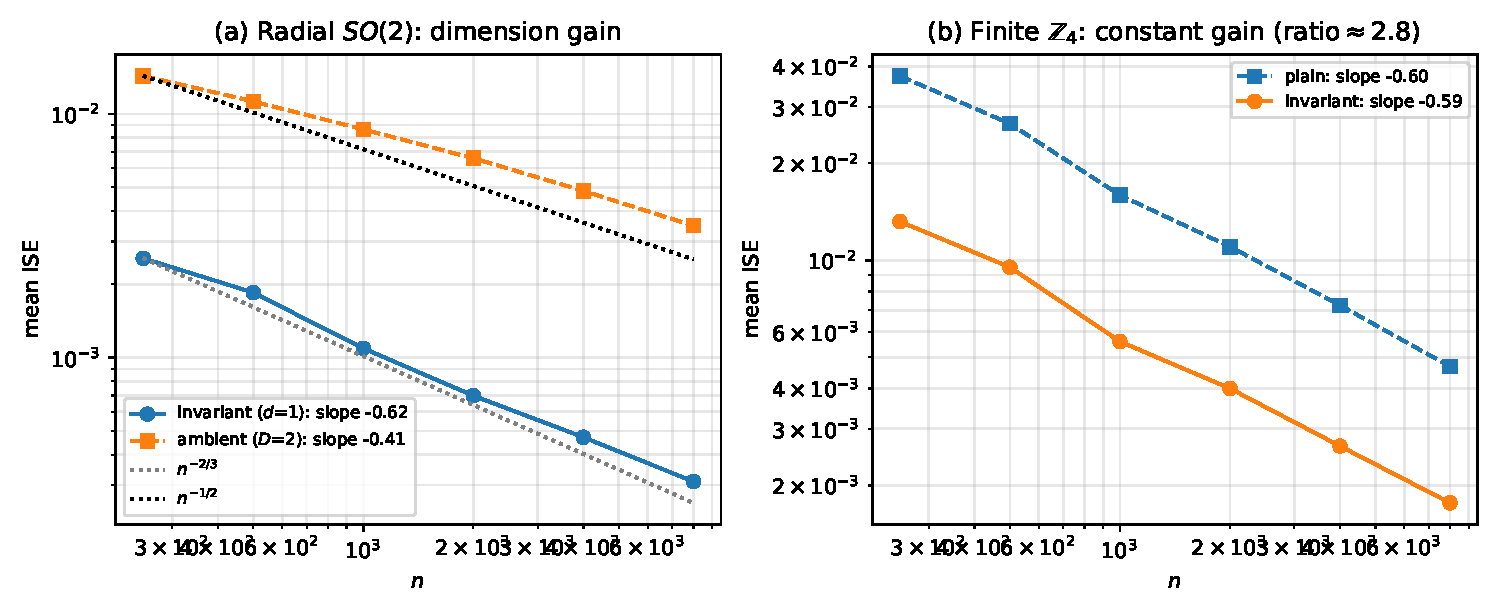
\includegraphics[width=\textwidth]{sim_invariant_minimax.pdf}
\caption{Penalised projection estimator. \textbf{(a)} Radial $SO(2)$: the
invariant estimator ($d=1$) decays at slope $-0.62\approx-2/3$, the ambient
estimator ($D=2$) at $-0.41\approx-1/2$ --- the effective-dimension gain.
\textbf{(b)} Finite $\mathbb Z_4$: equal slopes and an $n$-independent ISE ratio
$\approx2.8\le|G|$ --- a constant gain only, as predicted for $0$-dimensional
orbits. Produced by \texttt{sim\_invariant\_minimax.py}.}
\label{fig:sim}
\end{figure}

\paragraph{Reproducibility.}
Figure~\ref{fig:sim} and all reported slopes are produced by the single script
\texttt{sim\_invariant\_minimax.py} (Python; \texttt{numpy}, \texttt{scipy},
\texttt{matplotlib}), with a fixed seed (\texttt{numpy} generator seeded at
\texttt{20260619}). Running \texttt{python3 sim\_invariant\_minimax.py}
regenerates the figure \texttt{sim\_invariant\_minimax.pdf} and prints, for each
sample size $n\in\{250,500,1000,2000,4000,8000\}$, the mean integrated squared
errors and the fitted $\log$--$\log$ slopes; the radial experiment averages $30$
replications, the finite-group control $80$. No quantity in this section is set by
hand.

\section{Discussion}\label{sec:disc}

The two scope-limiting points of the additive and multiplicative analyses are now
\emph{assumptions} under which the theorems hold, rather than gaps. The stratified
case is covered by Assumption~\ref{ass:strata}: when the action is not free,
$M=E/G$ is an orbifold, but under Ahlfors $d$-regularity the singular strata are
$\mu_G$-null and the rate is governed by the top stratum $M_0$. What remains genuinely
open is a target whose smoothness interacts essentially with the singular locus
(local dimension varying across strata), which would call for a stratified
smoothness class. The multiplicative regime is covered by
Assumption~\ref{ass:phichart}: the conclusions require only chart regularity (a
compact $d$-regular region in the $\phi$-chart with the target bounded away from
$0$ and $\infty$ there), and \emph{no} tail condition on $X$, so genuinely
heavy-tailed positive/compositional data are admissible
(Remark~\ref{rem:heavyinstances}). The natural next step is to relax the compact
chart region to an unbounded one by controlling the integrability of $\log X$; the
information-theoretic route makes this plausible because the concentration step is
tail-free (Remark~\ref{rem:tailfree}), so the remaining work is
approximation-theoretic, on the quotient geometry, not probabilistic.

\begin{thebibliography}{99}

\bibitem{barroncover} A.~Barron and T.~Cover. Minimum complexity density
estimation. \emph{IEEE Trans.\ Inform.\ Theory}, 37(4):1034--1054, 1991.

\bibitem{barronbirgemassart} A.~Barron, L.~Birg\'e, and P.~Massart. Risk bounds for
model selection via penalization. \emph{Probab.\ Theory Related Fields},
113:301--413, 1999.

\bibitem{bietti2021} A.~Bietti, L.~Venturi, and J.~Bruna. On the sample complexity
of learning under geometric stability. In \emph{Advances in Neural Information
Processing Systems (NeurIPS)}, 2021.

\bibitem{birgemassart98} L.~Birg\'e and P.~Massart. Minimum contrast estimators on
sieves: exponential bounds and rates of convergence. \emph{Bernoulli},
4(3):329--375, 1998.

\bibitem{elesedy2021} B.~Elesedy and S.~Zaidi. Provably strict generalisation
benefit for equivariant models. In \emph{International Conference on Machine
Learning (ICML)}, 2021.

\bibitem{hendriks1990} H.~Hendriks. Nonparametric estimation of a probability
density on a Riemannian manifold using Fourier expansions. \emph{Ann.\ Statist.},
18(2):832--849, 1990.

\bibitem{li} J.~Q.~Li. \emph{Estimation of Mixture Models}. Ph.D.\ thesis, Yale
University, 1999.

\bibitem{massart} P.~Massart. \emph{Concentration Inequalities and Model
Selection}. Lecture Notes in Mathematics 1896. Springer, 2007.

\bibitem{pelletier2005} B.~Pelletier. Kernel density estimation on Riemannian
manifolds. \emph{Statist.\ Probab.\ Lett.}, 73(3):297--304, 2005.

\bibitem{tahmasebi2023} B.~Tahmasebi and S.~Jegelka. The exact sample complexity
gain from invariances for kernel regression. In \emph{Advances in Neural
Information Processing Systems (NeurIPS)}, 2023.

\bibitem{tsybakov} A.~B.~Tsybakov. \emph{Introduction to Nonparametric Estimation}.
Springer, 2009.

\bibitem{wongshen} W.~H.~Wong and X.~Shen. Probability inequalities for likelihood
ratios and convergence rates of sieve MLEs. \emph{Ann.\ Statist.}, 23(2):339--362,
1995.

\end{thebibliography}

\end{document}
